\section{What's Done and Left?}

\begin{frame}{Tasks}

DONE:
\begin{itemize}
    \item $\CheckedBox$  CMaxwellVariable class
    \item $\CheckedBox$  CMaxwellSolver class except for the BC part
    
    \begin{itemize}
        \item Solver Initialization: Initial variable state setting is quite easy compared to other solver's variables. Setting to zero initially is enough.
        
        \item Spatial Residual: flux-splitting method is categorized to be the source term, while the current density influence on $dE/dt$ is will also be added.
    \end{itemize}
    
    \item $\CheckedBox$  CNumerics class using flux-splitting method to compute residual
    \item $\CheckedBox$  CDriver class
    \item $\CheckedBox$  CIntegration class
\end{itemize}

\end{frame}

\begin{frame}{Tasks}
TODO:
\begin{itemize}
    \item $\Box$  BC part of the Solver class
    \begin{itemize}
        \item Non-reflection condition.
        \item PMR, perfect matched layer.
        \item Planar EM wave as source.
        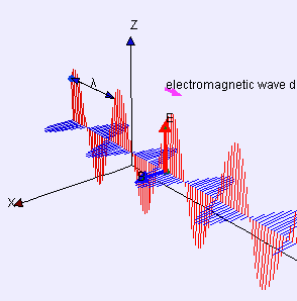
\includegraphics[width=0.2\linewidth]{figures/PlanarWave.png}
        \item Dielectric material, perfect conductor and perfect magnetized material.
    \end{itemize}
    \item $\Box$ Output function 
    \item $\Box$ Classical Test Scene Result Verification
    \item $\Box$ Thin-Wire model
    
    No similar concepts found in fluid dynamics.
\end{itemize}


\end{frame}


% \begin{frame}{Tasks}
% For the EM Maxwell module in unstructured mesh,
% \begin{itemize}
%     \item \emph{What's done?}
%     \begin{itemize}
%         \item Researched on the current stability analysis of the Maxwell flux instability.
%         \item Implemented the flux-splitting numerical method in SU2.
%     \end{itemize}
%     \item \emph{What's left?} 
%     \begin{itemize}
%         \item To implement the boundary condition flux computation.
%         \item To simulate the thin-witr model, which can be used to simulate the coil in tokamaks.
%         \item To couple different modules together.
%     \end{itemize}
% \end{itemize}


% For the magnetic reconnection simulation,
% \begin{itemize}
%     \item Maxwell module
%     \item Pressure module
%     \item Torus geometry setting
% \end{itemize}
% \end{frame}
